% !TEX root = ../main.tex
\chapter{车道汇合模型与群决策算法框架}
\label{cha:algorithm}
\section{车道汇合问题模型构建}
道路交汇口广泛存在于城市道路、高速公路中,是一种十分常见的交通场景。交汇的两条道路通常分为主路和辅路。其中主路通常有多条车道,路面较宽敞,车速快;辅路通常只有一条车道,车速较慢。按照我国现行交通法规,辅路车辆应在不影响主路车辆正常通行的情况下汇入主路。在主路车流密集,车速较高时,往往会造成辅路车辆停车等待的情况,带来了道路资源、燃油的浪费。若通过交汇口的车辆均由 CAV 构成,则有可能通过群体性的决策使交汇过程无需停车,同时减小通行时间和燃油损耗。

考虑如图\ref{fig:merge}所示的交汇路口。为了简化问题,考虑主路只有一条车道的情况。可能发生横向碰撞的区域成为交汇区,长度为$S$
。在控制区内,车辆之间、车辆与中央控制器之间允许交换信息并运行控制算法, 控制区起点
到交汇区起点的长度为$L$。
\begin{figure}[htbp]
\centering
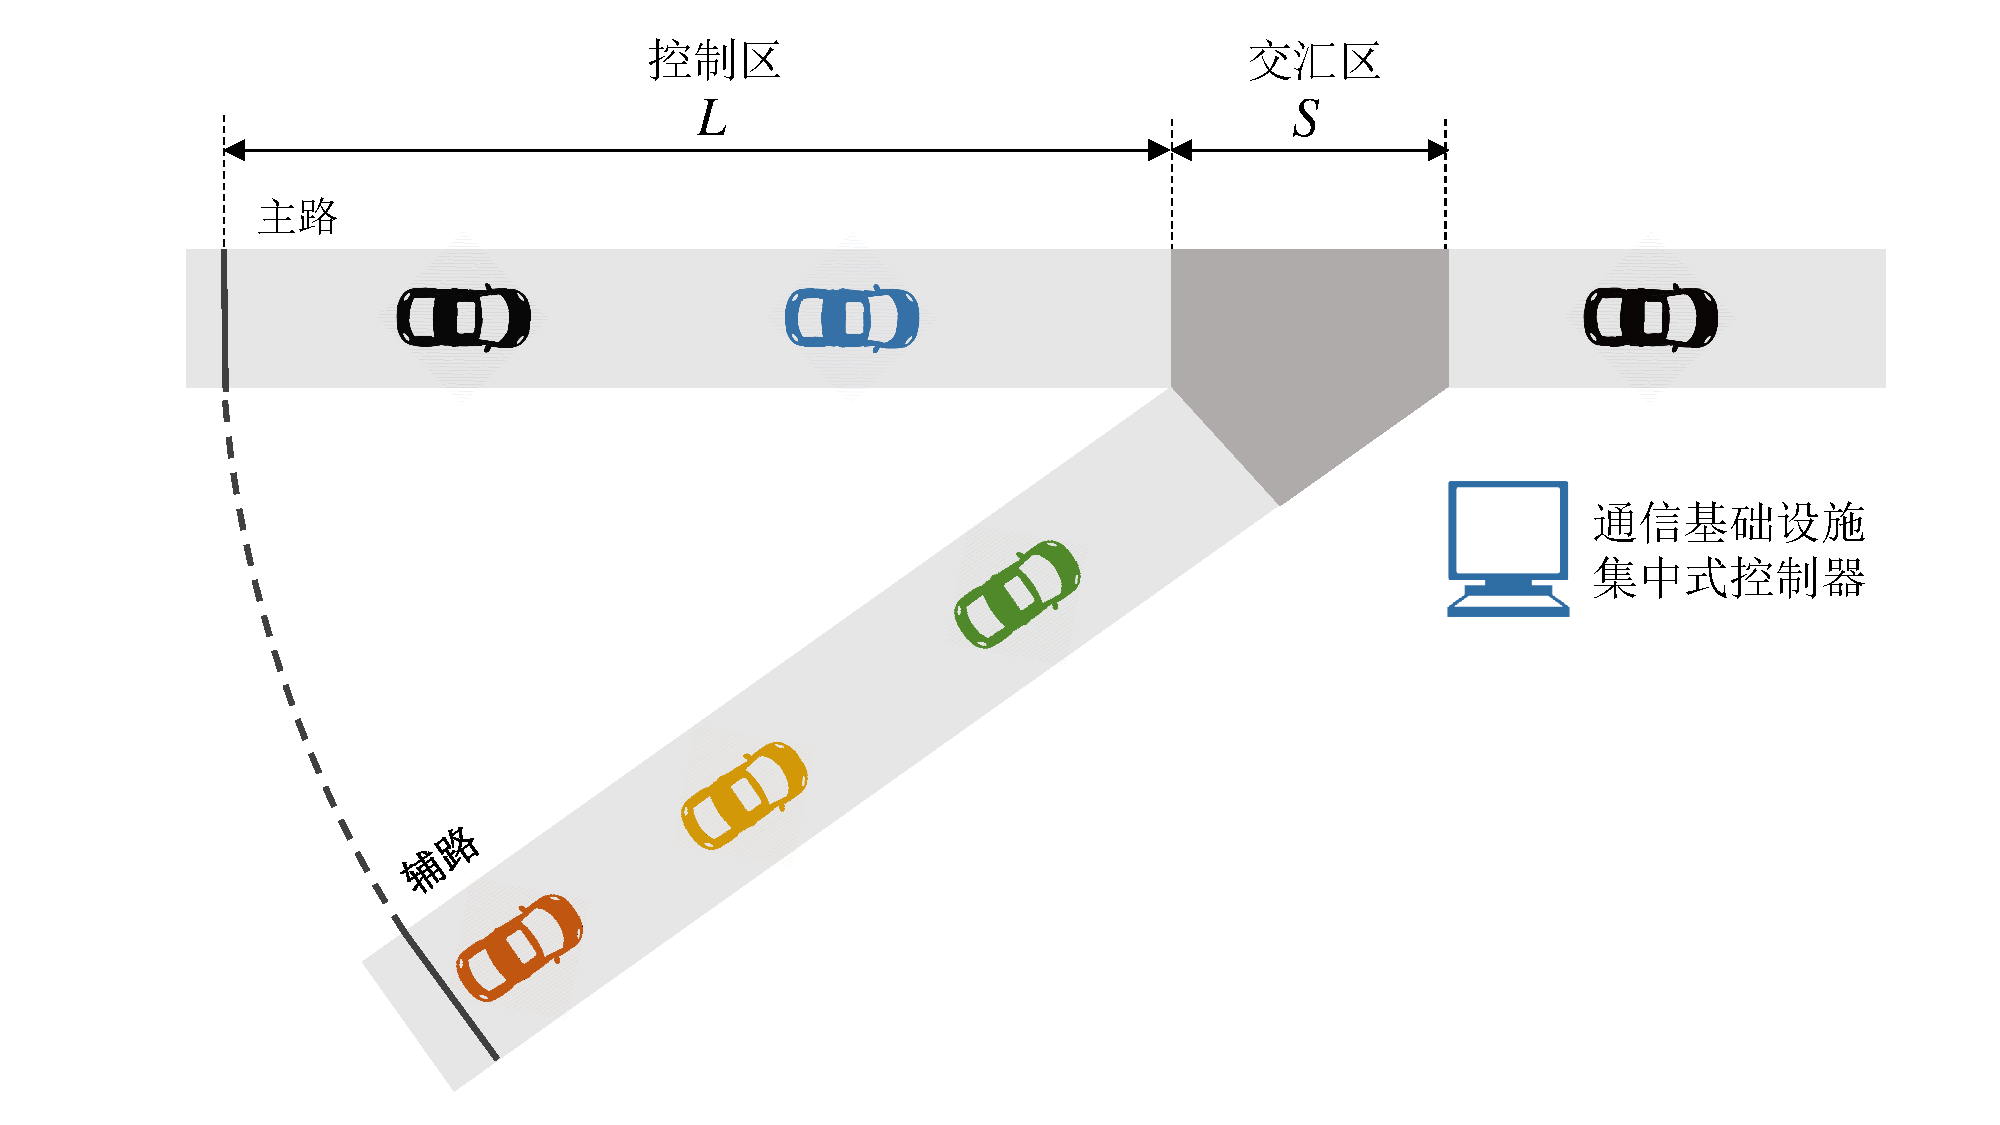
\includegraphics[width=14cm]{../figures/merge.pdf}
\caption{交汇路口示意图}
\label{fig:merge}
\end{figure}

\subsection{车辆状态方程}
假设在时刻 $t$时,位于控制区内的车辆具有某种编号 $\mathcal{N}(t)={1,\dots,N(t)}$,其中 $N(t)$为 $t$时刻控制区内车辆总数。对于每辆车$i\in \mathcal{N}(t)$,系统状态方程为
\begin{equation}
\dot{\bm{x}}_i=f(t,\bm{x}_i,u_i),\quad \bm{x}_i(t_i^0)=\bm{x}_i^0,
\end{equation}
其中$\bm{x}_i(t)$,$u_i(t)$分别为第$i$辆车在$t$时刻的状态量和控制量。对于本课题讨论的无人车控制,假定车辆的轨迹已经确定,无需控制方向,只需控制速度。为了保证速度的连续性,选取控制量为加速度,则控制量与状态量的关系为,
\begin{equation}
\begin{gathered}
\dot{p}_i=v_i(t),\\
\dot{v}_i=u_i(t),
\end{gathered}
\label{eq:state}
\end{equation}
其中 $p_i(t)\in \mathcal{P}_i$,$v_i(t)\in \mathcal{V}_i$,$u_i(t)\in \mathcal{U}_i$分别为第 $i$辆车在 $t$时刻的位置,速度和加速度。由于轨迹事先已确定,只需要两个标量 $p_i$与 $v_i$即可确定当前车辆的位置和速度。二者构成了车辆的状态向量 $\bm{x}_i(t)=[p_i(t), v_i(t)]^\mathrm{T}\in \mathcal{X}_i$,$\mathcal{X}_i=\mathcal{P}\times\mathcal{V}$,并定义进入控制区的初始状态为$\bm{x}_i^0 = [0, v_i^0]^\mathrm{T}$。

对于实际运行的车辆,其速度和加速度均有限,表达为以下约束,
\begin{equation}
\begin{aligned}
u_{i,\min}\leq u_i(t)\leq u_{i,\max}&, \quad \text{and}\\
0\leq v_{\min}\leq v_i(t)\leq v_{\max}&, \quad \forall t\in[t_i^0, t_i^\mathrm{f}],
\end{aligned}
\label{eq:single_constraint}
\end{equation}
其中 $t_i^\mathrm{f}$为第 $i$辆车离开交汇区的时刻,即控制算法结束的时刻。 $u_{i,\min}$,$u_{i,\max}$分别为第$i$辆车的最小、最大加速度,$v_{\min}$,$v_{\max}$为道路的最低、最高限速。为简单起见,考虑同质车辆,所有CAV均具有相同的最小、最大加速度,即$u_{i,\min}=u_{\min}$,$u_{i,\max}=u_{\max}$。

\subsection{安全性约束与假设}
上一节建立了每辆车的状态方程和单车的约束条件,本节考虑车辆之间的约束关系。

控制算法首先要保证车辆之间不发生追尾。对同一车道上的车辆,定义安全距离$\delta < S$,同车道车辆之间不追尾的约束可以表示为,
\begin{equation}
s_i(t)=p_k(t)-p_i(t)\geq \delta, \ \forall t\in [t_i^0, t_i^\mathrm{f}],
\label{eq:colli_rear}
\end{equation}
其中$k$表示与$i$在同一车道的前一辆车的编号。上式涵盖了控制区、交汇区不发生同车道追尾的约束条件。

车辆仅在交汇区可能与对路车辆发生横向碰撞。给出如下定义:
\begin{definition}[可能碰撞集]
对所有$i\in \mathcal{N}(t)$,定义第 $i$辆车的{\heiti 可能碰撞集} $\Gamma_i$为可能发生横向碰撞的$i$车位置构成的集合,即
\begin{equation}
\Gamma_i\triangleq \{p_i(t)\in[L,L+S],\  \forall t\in [t_i^\mathrm{m},t_i^\mathrm{f}]\}.
\end{equation}
其中$t_i^\mathrm{m}$为第$i$辆车离开控制区,进入交汇区的时刻。
\end{definition}
为了避免横向碰撞,对任意不在同一条路上的两辆车 $\forall i,j\in \mathcal{N}(t)$,给出如下约束:
\begin{equation}
\Gamma_i\cap \Gamma_j=\varnothing, \ \forall t\in [t_i^\mathrm{m},t_i^\mathrm{f}].
\label{eq:colli_lateral}
\end{equation}
上式要求来自相互交汇的两条路上的车辆不能同时出现在交汇区。这个约束必能保证车辆在交汇区不发生横向碰撞,但当交汇区的长度很长时,约束可能过强,没有必要。在下面的章节中将讨论如何放松该约束。

在定义优化目标之前,对控制算法做以下假设。
\begin{assumption}
进入控制区的车$i$满足约束式\eqref{eq:single_constraint},式\eqref{eq:colli_rear}。
\label{ass:restrict}
\end{assumption}
\begin{assumption}
CAV在交汇区保持匀速行驶,且速度相同,即$v_i(t) = v_i(t_i^\mathrm{m}) = v_i(t_i^\mathrm{f}) = v_\mathrm{d}, \ \forall t\in [t_i^\mathrm{m},t_i^\mathrm{f}]$,其中$v_\mathrm{d}$为期望速度。由此可得
\begin{equation}
t_i^\mathrm{f}=t_i^\mathrm{m} + \frac{S}{v_\mathrm{d}}.
\end{equation}
\label{ass:smooth}
\end{assumption}
\begin{assumption}
忽略CAV之间信息传输的延时和错误。
\label{ass:time}
\end{assumption}

在以上假设中,假设\ref{ass:restrict}保证了初始状态的可行性。假设\ref{ass:smooth}忽略了交汇区的速度变化,且假设车辆在进入交汇区之前已经调整到了期望速度$v_\mathrm{d}$。该速度可以根据路段的限速事先给定。这是为了方便讨论交汇区的不碰撞约束,实际情况与此有一定差别。后文将对此展开进一步讨论。假设\ref{ass:time}保证车辆之间信息交互是实时且准确的。但本文的模型在信息的延时和错误处于有限范围内,仍可进行扩展。

\section{群决策算法框架}
本节运用上一节讨论的安全性假设建立车辆之间的时间约束关系,给出通行时间下界序列的确定方法,并提出最小化控制量输入的目标函数。之前的车辆交汇口控制文献通常都只针对安全性和通行目标函数之中的一个进行研究,本文的算法框架将二者结合,并在保证安全的前提下对通行时间也同时进行了优化。
% 这里加一段优化目标的综述
\subsection{时间序列的确定}
\label{ssec:time_series}
\textbf{由安全性约束确定界限}
\ \ 在假设\ref{ass:smooth}下,考虑到约束式\eqref{eq:colli_rear}与式\eqref{eq:colli_lateral},可以由$t_{i-1}^\mathrm{m}$确定$t_i^\mathrm{m}$的下界$(t_i^\mathrm{m})^*$,实际进入交汇区的时间$t_i^\mathrm{m}$应满足$t_i^\mathrm{m} < (t_i^\mathrm{m})^*$。定义以下两个集合:
\begin{definition}
定义$\mathcal{L}_i$为与$i$车在同一车道的车编号的集合,$\mathcal{C}_i$为与$i$车在不同车道的车编号的集合。
\end{definition}
由交汇口场景可知,$i-1$车必属于以上两个集合之一。考虑以下两种情况:
\begin{enumerate}[label=(\arabic*), wide=\parindent]
% \begin{enumerate}
\item $i-1\in \mathcal{L}_i$,此时前后车只需保持安全距离,当$i-1$车驶过$\delta$距离后,$i$车便可进入交汇区。由此可得,
\begin{equation}
(t_i^\mathrm{m})^*=t_{i-1}^\mathrm{m} + \frac{\delta}{v_\mathrm{d}}.
\label{eq:t_case1}
\end{equation}
\item $i-1\in \mathcal{C}_i$,由式\eqref{eq:colli_lateral},当$i-1$车完全驶过交汇区后,$i$车才能进入交汇区。由此可得,
\begin{equation}
(t_i^\mathrm{m})^*=t_{i-1}^\mathrm{m} + \frac{S}{v_\mathrm{d}}.
\label{eq:t_case2}
\end{equation}
\end{enumerate}

上述情况二满足了式\eqref{eq:colli_lateral}所要求的不同车道不同时出现在交汇区的要求。若交汇区比较长,该要求可以适当放松为,使不同车道间车辆交汇后相距为 $r < S$,$r$为不同车道保证不发生横向碰撞的安全距离。在实际道路条件下,安全距离应随着速度的增加而适当增大。由于交汇区车速仍可视为保持期望速度 $v_\mathrm{d}$,$r$也可以作为常数而预先确定下来。情况二对应的时间关系变为,
\begin{equation}
(t_i^\mathrm{m})^*=t_{i-1}^\mathrm{m} + \frac{r}{v_\mathrm{d}}.
\label{eq:t_case2r}
\end{equation}

另外,对于不存在前车的第一辆车,其到达交汇区时间 $t_1^\mathrm{m}$可由优化目标解出。这将在下文进一步讨论。

\textbf{由状态量控制量限制确定界限}
\ \ 由于车辆的速度和加速度满足约束式\eqref{eq:single_constraint},某辆车自身具有通过控制区的最短时间。可分以下三种情况:
\begin{enumerate}[label=(\arabic*), wide=\parindent]
% \begin{enumerate}
\item 车辆以最大加速度运行至最大速度,之后保持最大速度行驶一段时间,再以最大加速度减速至期望速度$v_\mathrm{d}$,恰好在速度减至$v_\mathrm{d}$时到达交汇区,如图\ref{fig:vmax}。
\begin{figure}[htbp]
\centering
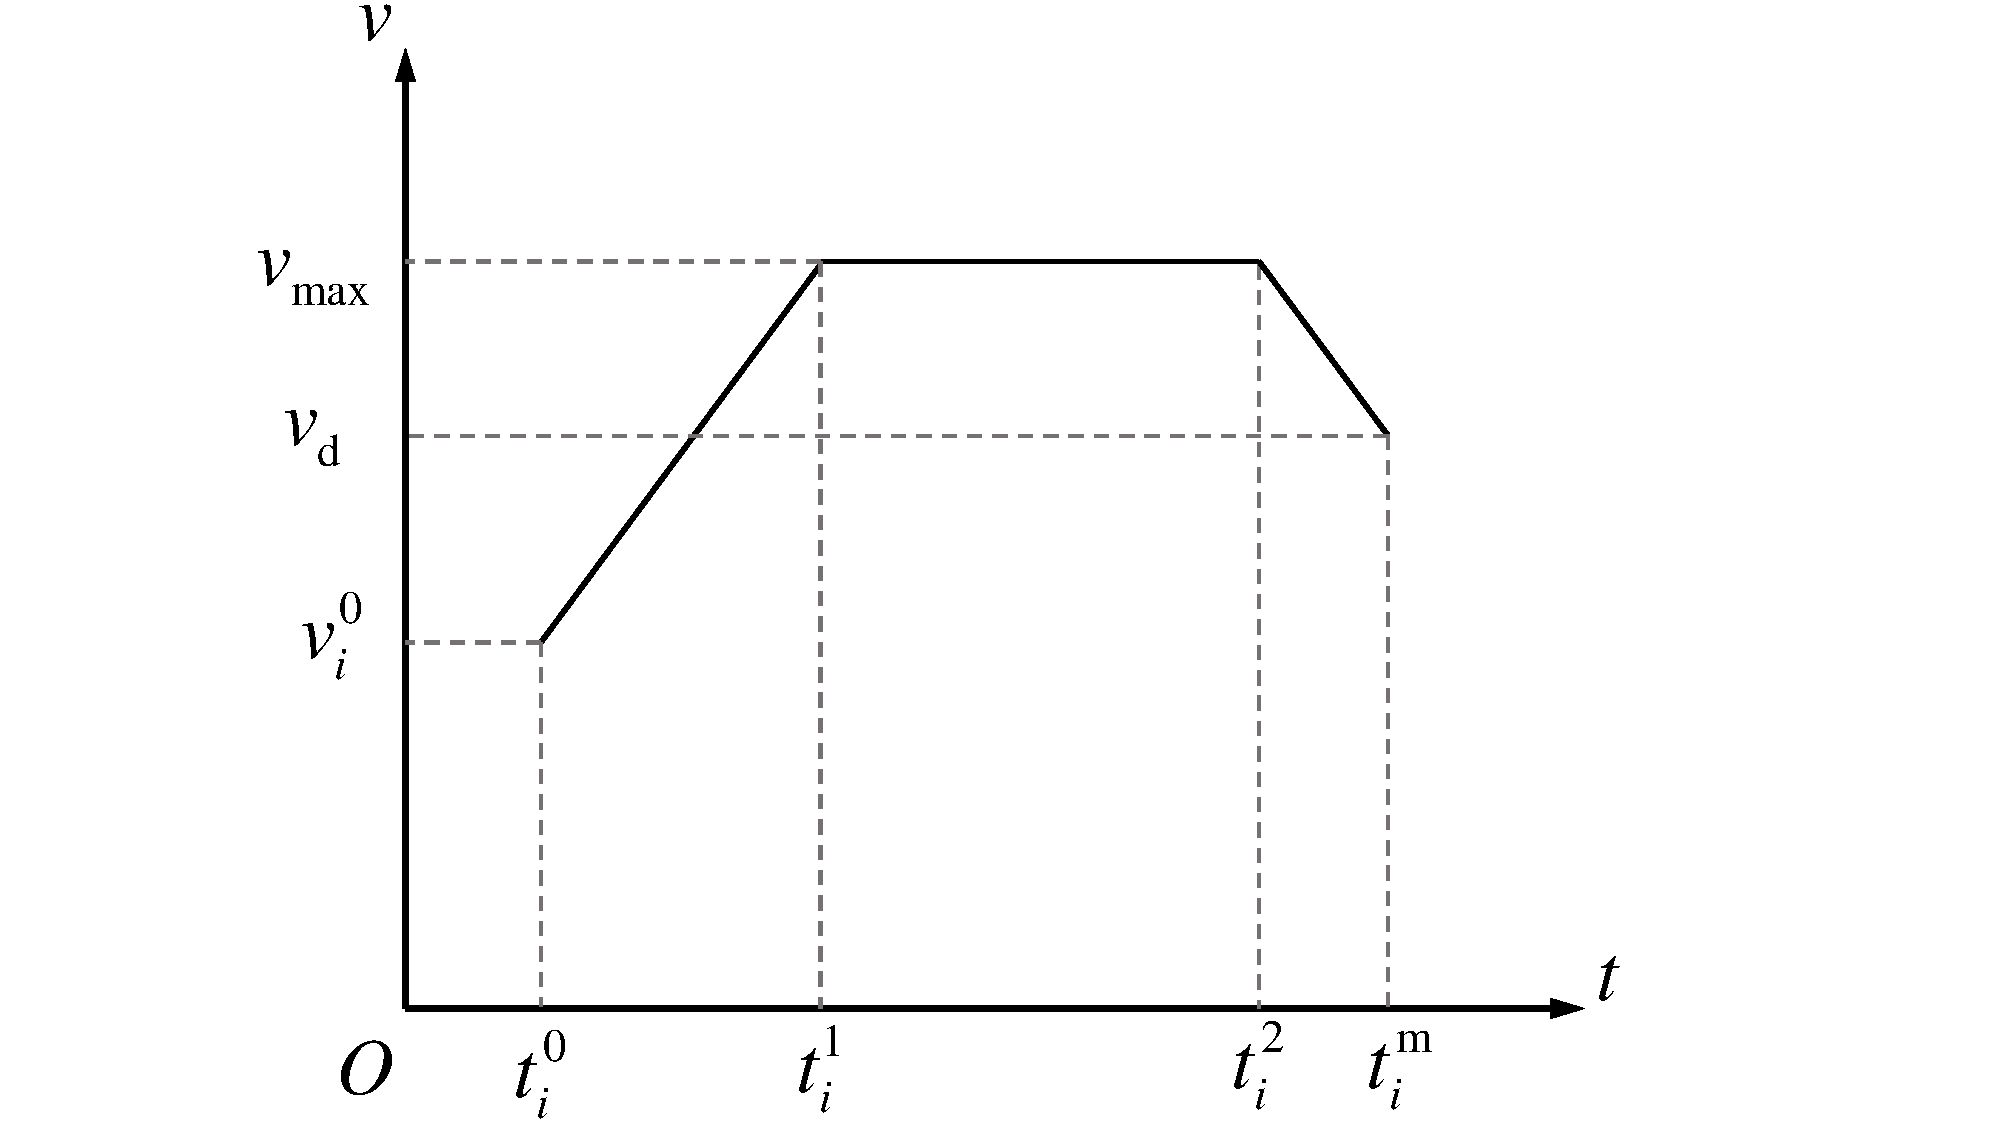
\includegraphics[width=12cm]{figures/vmax.pdf}
\caption{达到最大速度的速度-时间关系图}
\label{fig:vmax}
\end{figure}

由图可得方程
\begin{gather}
u_{\max}(t_i^1-t_i^0)=v_{\max}-v_i^0,\\
u_{\max}(t_i^\mathrm{m}-t_i^2)=v_{\max}-v_\mathrm{d},\\
\frac12(v_{\max}+v_i^0)(t_i^1-t_i^0) + v_{\max}(t_i^2-t_i^1) + \frac12(v_{\max}+v_\mathrm{d})(t_i^\mathrm{m}-t_i^2) = L.
\end{gather}
解得
\begin{equation}
(t_i^\mathrm{m})^* = t_i^0 + \frac{L}{v_{\max}} + \frac{v_{\max}-v_i^0-v_\mathrm{d}}{u_{\max}} + \frac{(v_i^0)^2+(v_\mathrm{d})^2}{2u_{\max}v_{\max}}.
\label{eq:ts:tm1}
\end{equation}
注意在这种情况下未必有$v_i^0 > v_\mathrm{d}$,例如车辆可能直接以最大速度进入控制区,则$t_i^1=t_i^0$,式\eqref{eq:ts:tm1}仍然成立。

\item 车辆以最大加速度运行,但未达最大速度即减速,并在速度恰好减至$v_\mathrm{d}$时到达交汇区,如图\ref{fig:vmed}。
\begin{figure}[htbp]
\centering
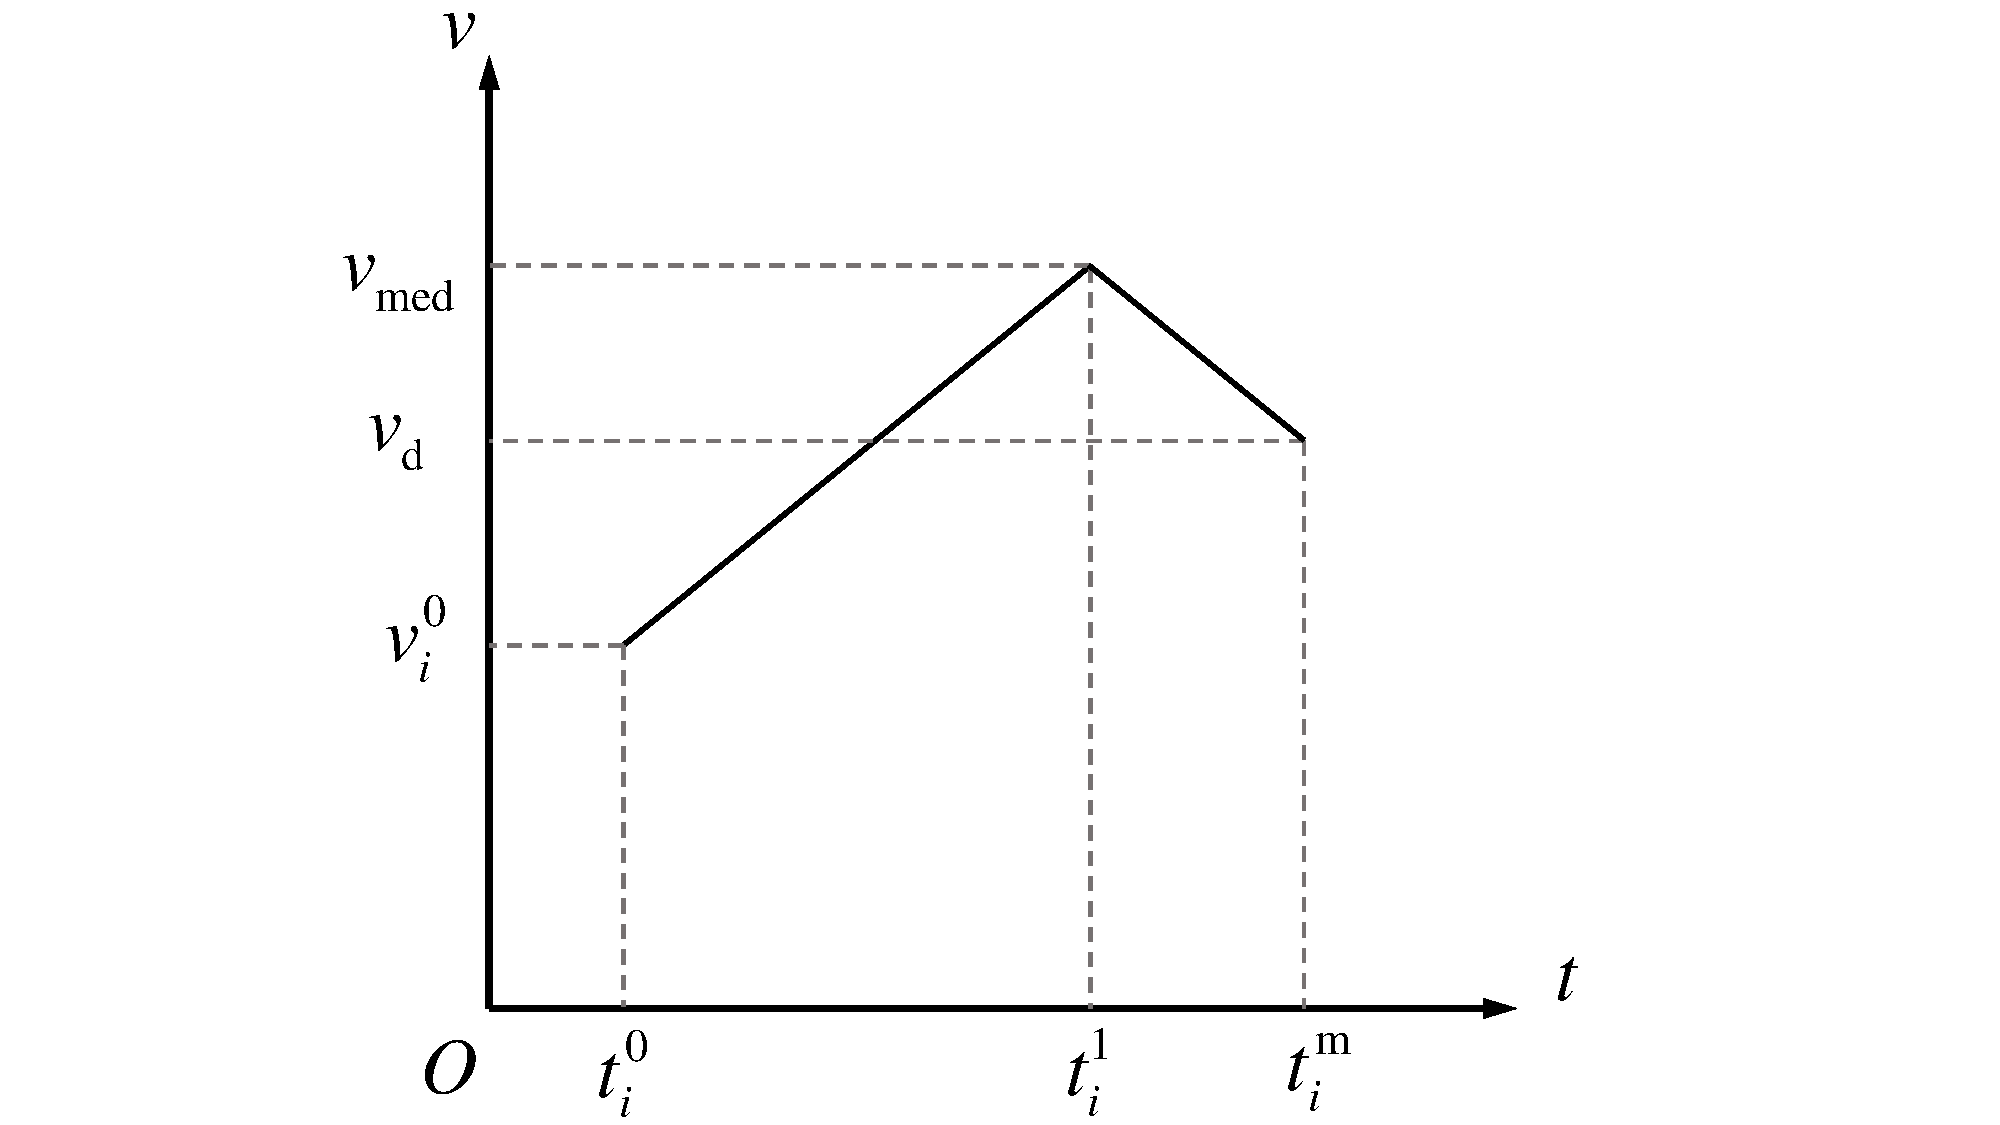
\includegraphics[width=12cm]{figures/vmed.pdf}
\caption{未达到最大速度的速度-时间关系图}
\label{fig:vmed}
\end{figure}

由图可得方程
\begin{gather}
u_{\max}(t_i^1-t_i^0)=v_\mathrm{med}-v_i^0,\\
u_{\max}(t_i^\mathrm{m}-t_i^1)=v_\mathrm{med}-v_\mathrm{d},\\
\frac12(v_\mathrm{med}+v_i^0)(t_i^1-t_i^0) + \frac12(v_\mathrm{med}+v_\mathrm{d})(t_i^\mathrm{m}-t_i^1) = L.
\end{gather}
解得
\begin{equation}
(t_i^\mathrm{m})^*=t_i^0+\frac{\sqrt{2(2u_{\max}L+(v_i^0)^2+v_\mathrm{d}^2)}-v_i^0-v_\mathrm{d}}{u_{\max}}.
\end{equation}
\item 除以上两种情况外,还有可能车辆以最大加速度运行,但还未达到期望速度即到了交汇区。这种情况可以通过给定足够长的控制区来避免。控制区的长度$L$应足够车辆从最小速度$v_{\min}$以最大加速度$u_{\max}$达到最大速度$v_{\max}$,可得
\begin{equation}
L\geq \frac{v_{\max}^2-v_{\min}^2}{2u_{\max}}.
\end{equation}
这样在计算时间下界时只需考虑前两种情况。
\end{enumerate}

综合以上几种$t_i^\mathrm{m}$的确定方法,给出如下定理。
\begin{theorem}
在预先确定的某种通行顺序下,车辆到达交汇口时间的下界可由下式迭代确定,
\begin{equation}
t_i^\mathrm{m}=
\begin{dcases}
t, & \text{if}\quad i=1,\\
\max \left\{t_{i-1}^\mathrm{m} + \frac{\delta}{v_\mathrm{d}}, t_i^\mathrm{c}\right\}, & \text{if}\quad i-1\in \mathcal{L}_i,\\
\max \left\{t_{i-1}^\mathrm{m} + \frac{S}{v_\mathrm{d}}, t_i^\mathrm{c}\right\}, & \text{if}\quad i-1\in \mathcal{C}_i,
\end{dcases}
\label{eq:tmcase}
\end{equation}
其中,
\begin{align}
t_i^\mathrm{c}&=t_i^{m,1}\mathds{1}_{v_i^\mathrm{m}=v_{\max}}+t_i^\mathrm{m,2}(1-\mathds{1}_{v_i^\mathrm{m}=v_{\max}}),\label{eq:alg:case}\\
t_i^\mathrm{m,1}&=t_i^0 + \frac{L}{v_{\max}} + \frac{v_{\max}-v_0-v_\mathrm{d}}{u_{\max}} + \frac{v_0^2+v_\mathrm{d}^2}{2u_{\max}v_{\max}},\\
t_i^\mathrm{m,2}&=t_i^0+\frac{\sqrt{2(2u_{\max}L+v_0^2+v_\mathrm{d}^2)}-v_0-v_\mathrm{d}}{u_{\max}}.
\end{align}
上式中$v_0 = v_i^0$。
\end{theorem}

由式\eqref{eq:tmcase}可在进入路口前即确定每辆车$t_i^\mathrm{m}$的下界,若能选择合适的控制策略使车辆恰好在下界时间点到达交汇口,即在某种通过顺序下使旅行时间达到了最优。实际运算中不需要按照式\eqref{eq:alg:case}做判断,只需取$t_i^{m,1}$与$t_i^{m,2}$中较大的即可。

\subsection{优化目标建立}
研究CAV的决策问题,就是在控制量满足一定约束的情况下,对每辆车给出一列控制量输入$u_i(t)$对于车道汇合的场景,一般优化目标包含最小化控制量的输入和最小化平均通行时间。\cite{Rios2016Automated}将二者包含在同一目标函数中,表达为,
\begin{equation}
\begin{aligned}
&\min_{u_i\in \mathcal{R}_i}\left(w_1\frac12\sum^{N(t)}_{i=1}\int_{t_i^0}^{t_i^\mathrm{f}}C_i\left(u_i\left(t\right)\right)\mathrm{d}t + w_2\sum_{i=2}^{N(t)}|t_i^\mathrm{m}(u_{(1:i)}(t))-t_{i-1}^\mathrm{m}(u_{(1:i-1)}(t))|\right),\\
&
\begin{aligned}
\text{Subject to:} & \quad \mbox{\eqref{eq:state}}, \quad \forall i\in \mathcal{N}(t),\\
& \quad \mbox{\eqref{eq:colli_lateral}}, \quad \forall i,j \in \mathcal{N}(t), i\neq j.
\end{aligned}
\end{aligned}
\label{eq:two_item_obj}
\end{equation}
其中$w_1$,$w_2$为调整两项权重的比例系数,$t_i^\mathrm{m}(u_{(1:i)}(t))$表示$i$车的$t_i^\mathrm{m}$可能与之前所有车的控制量输入都有关。$\mathcal{R}_i$定义如下:
\begin{definition}[控制区间]
对每辆车$i$,定义该车的{\heiti 控制区间} $\mathcal{R}_i$为,
\begin{equation}
\begin{gathered}
\mathcal{R}_i\triangleq\{u_i(t)\in[u_{\min}, u_{\max}]\ |\ p_i(t)\leq p_k(t)-\delta, v_i(t)\in[v_{\min}, v_{\max}],\\
\forall i \in \mathcal{N}, |\mathcal{N}(t)|>1, \forall t \in [t_i^0, t_i^\mathrm{f}]\ \}.
\end{gathered}
\end{equation}
\label{def:possible_u}
\end{definition}
定义\ref{def:possible_u}给出了可能的控制量输入集合。

式\eqref{eq:two_item_obj}的第一项表示由控制量输入造成的损失,$C_i(u_i(t))$为控制量输入$u_i(t)$的某种函数。第二项为前后车进入交汇区时间差之和,该值越小,交汇路口吞吐量就越大。对于本文的优化问题,假设所有车辆均按照式\eqref{eq:t_case1},式\eqref{eq:t_case2}(或式\eqref{eq:t_case2r})确定的时间下限通行,则可以略去目标函数式\eqref{eq:two_item_obj}中的时间相关项,保留控制量相关项。选取目标为最小化控制量输入的平方\cite{Malikopoulos2016A,Rios2016Automated},即
\begin{equation}
J(\bm{u})=\frac12\int_{t_i^0}^{t_i^\mathrm{m}}u_i^2\mathrm{d}t,
\label{eq:one_item_obj}
\end{equation}
其中$\bm{u}$为所有车控制量输入函数构成的向量。在本文中控制量只有加速度。